\section{A reachable resource-objective gain without new scientific output}
\label{sec:native-terminal-cost}

The closed free-system search establishes no advantage over its strong visible
parent, but does not establish that parent as a world-level optimum.
We next execute the terminal-cost hypothesis described in
Section~\ref{sec:native-topic-system-search}, rather than increasing the same
search budget. This separate, development-informed control study tests a
reachable difference under the already declared $L_C=L_U+0.1K$. It is not
automatic institution invention, a comparison of optimizers or unused evaluation.
No designer proposes either program, and no objective is replaced after its
outcome is observed.

\paragraph{Exactly two source-defined controls.}
Both fresh worlds use the same four-year original simulation, five initial
researchers, openly reused development seed 61001, fixed Qwen3-8B scientists,
offline 103,107-paper corpus and original production, funding and annual costs.
Both inherit the core-plus-directly-related topic rule, original topic content
and durations, workflow-v5 authority, graph, ports, schedules and other source.
The reference retains its existing liquidity rule. The control changes only
that producer's Python body: after final-year publication and funding, but
before native annual costs, it transfers each other active researcher's
positive balance into the richest existing active researcher (lexical ID
breaks a balance tie). Transfers conserve resources; neither new money,
researchers, papers, graph edges nor a cost exemption is introduced.

The final-year intervention exploits a distinction in the unchanged native
resource consumer. A transfer leaving exactly zero does not deactivate its
donor. The subsequent negative annual charge clips the balance at zero and
deactivates that researcher. Requested negative charges and collected debits
therefore differ. This is an exercised original-world path, not a numerical
replacement of researchers or a new activity-cost law.

\paragraph{Normal completion and measured outcomes.}
The original writer exits normally with both scheduled worlds complete in
1,952.56 seconds (32m32.56s) on the shared local host. This elapsed interval is
not a dedicated GPU-speed benchmark. Two original-source/physical audits and
two cost projections match; two independently invoked readout exports match
in all three files. Both controls' full 179 scientist request payloads and
literal response choices are identical in order, with no unmatched requests.
All 36 accepted year/paper/content records are common, and their exact centered
opinion sum is $86/3$. Equal observed inputs/choices are not equivalence of
the two programs or an independent replication of researcher behavior.

\begin{table}[t]
\centering\small
\caption{Actual two-control outcomes. Lower loss is better. $K$ is collected
native activity cost, $Q$ unpaid activity cost and $R=K+Q$ requested expense.
The last two columns are measured terminal snapshots, not eligibility gates.}
\label{tab:native-terminal-cost}
\setlength{\tabcolsep}{4pt}
\begin{tabular}{lrrrrrrrr}
\toprule
Hand control & $L_T$ & $L_U$ & $L_C$ & $K$ & $Q$ & $R$ & Active & Balance\\
\midrule
Reference & $-36$ & $-28.67$ & $-8.67$ & 200 & 0 & 200 & 5 & 30\\
Consolidation & $-36$ & $-28.67$ & $-12.67$ & 160 & 40 & 200 & 1 & 70\\
\bottomrule
\end{tabular}
\end{table}

Annual collected expense is 50 in both worlds for years 1--3. At the final
handoff each world has 80 resource units. The control's four actual transfers,
11 units each, leave 80 in one existing researcher and zero in the other four.
Final-year collection is 10 rather than 50; requested annual expense remains
50, and the other 40 is unpaid. Closing active researchers are one versus five
and total remaining resources are 70 versus 30. All transfer receipts and
annual actor/ledger reconciliation are retained, without an attrition or
unpaid-expense veto.

\paragraph{A real declared-loss gain, not real efficiency.}
The measured $L_C$ improvement is exactly four units:
\[
 \Delta L_C=\Delta L_U+0.1\Delta K=0+0.1(-40)=-4.
\]
Thus this study supplies a feasible lower $L_C$ than the prior strong parent,
without improving the recorded output count or content opinions. For
interpretation only, define the requested-cost accounting diagnostic
$D_R=L_U+0.1(K+Q)$. Then
\[
 \Delta D_R=\Delta L_C+0.1\Delta Q=-4+4=0.
\]
$D_R$ is not optimized, substituted for the loss, used to select a program or
used to disqualify this gain. Requested native charges are themselves an
accounting instrument, not independently validated real-world resource use.
The observed gain is collection avoidance at the horizon, not reduced
requested expense, better science or demonstrated long-run welfare.
No fifth-year continuation is evaluated here.

\begin{figure}[t]
\centering
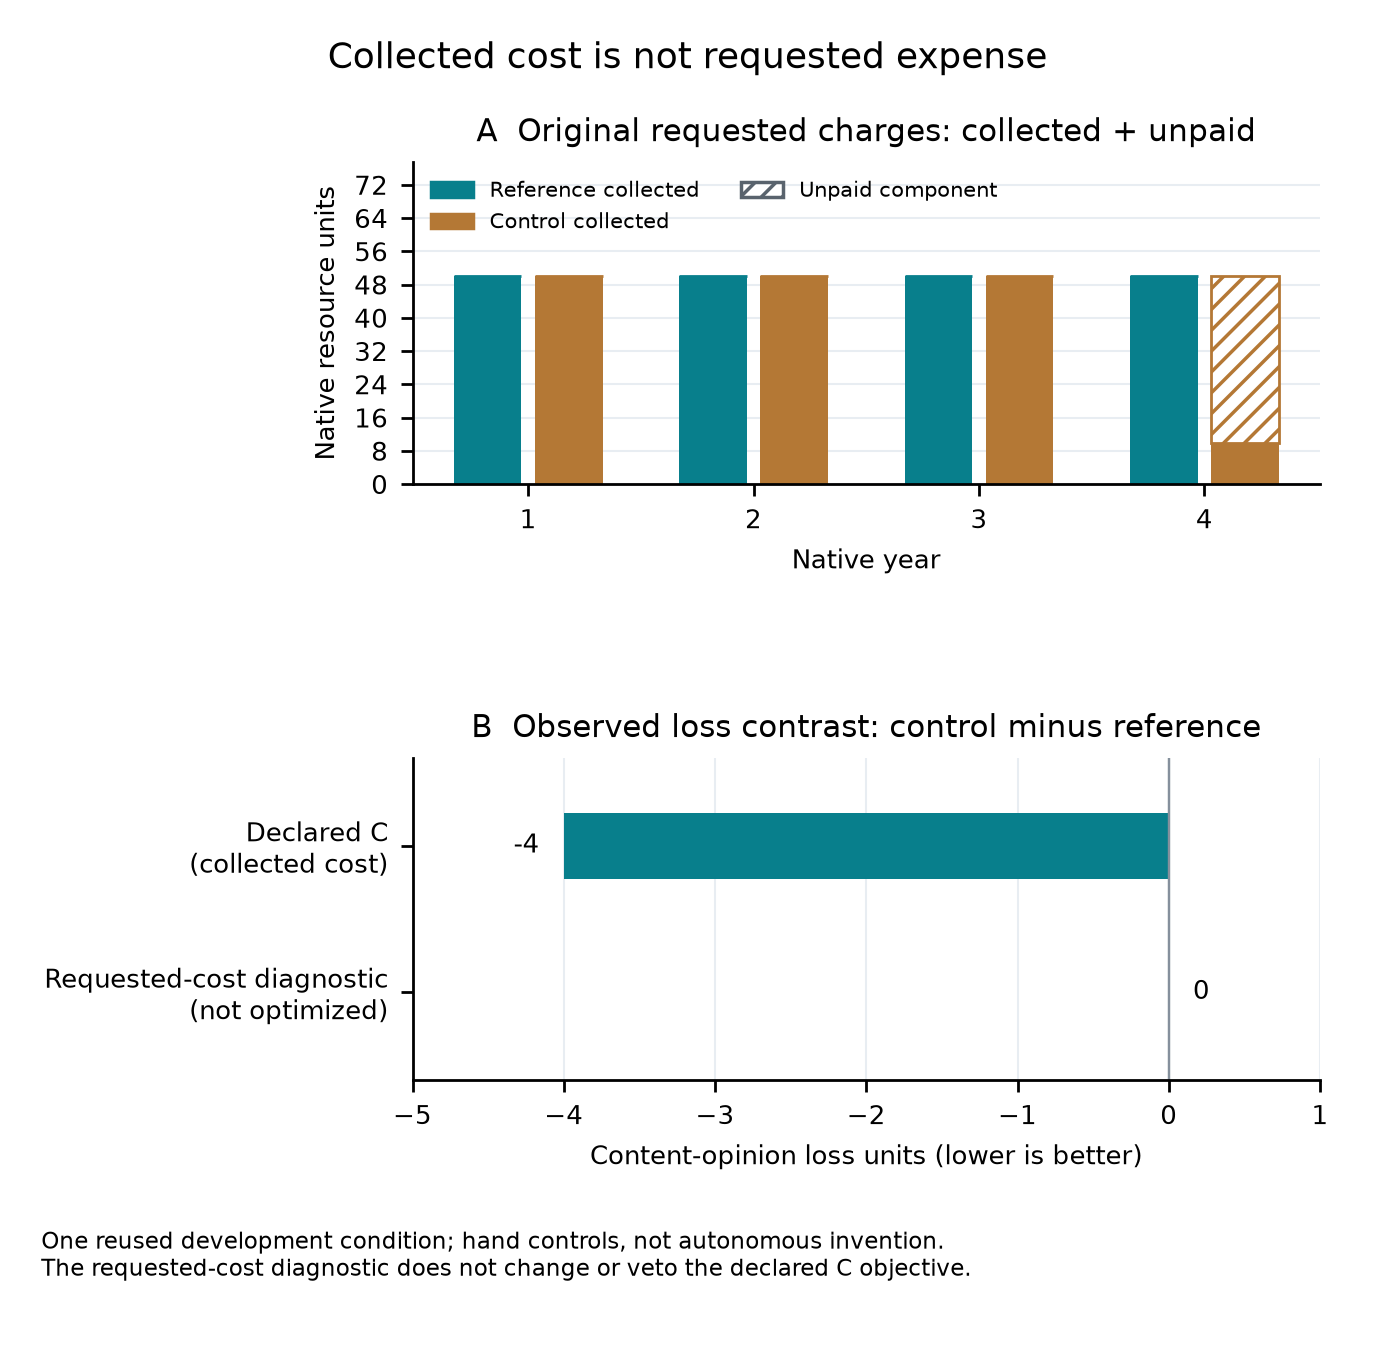
\includegraphics[width=\linewidth]{figures/native-terminal-cost-v1/collected-versus-requested.png}
\caption{Original annual expense and the loss contrast. Hatched segments are
unpaid charges, not saved requested work. The four-unit declared $L_C$ gain
vanishes in the separately labelled requested-cost diagnostic; the declared
objective and original outcomes remain unchanged. One reused development
condition and hand-authored controls provide no optimizer confidence interval.}
\label{fig:native-terminal-cost}
\end{figure}

\paragraph{Separate computational costs and research consequence.}
The physical caches contain 358 completed scientist responses, 537,104 input
and 32,382 output tokens, with a reported cached-input subset of 79,402 (not
added to the input total). The fixed content observer makes 108 physical POSTs,
using 48,375 input and 15,337 output tokens. Cache reuse across the identical
accepted records is not another physical rating. Two scientist-load attempts
have missing token usage, which remains unknown. There are no proposal,
designer-readiness or institutional extra-scientist calls in this hand study.
These inference measurements are separate from native resource units $K$;
they are not measured FLOPs, energy or monetary expense.

This contrast rejects a global-$L_C$-optimality interpretation of the previous
parent on this condition. It does not show that the local designer could
discover the mechanism, that a new topology is necessary or that code-defined
search is superior to a strong simple rule. It also does not create a strict
T/U preference reversal: these two objectives tie. The next free-system study
must distinguish available design authority, actual native consumer effects,
objective opportunity and discovery under matched information and budgets.
Elementary end-horizon accounting and reconstruction alone are not an
important main-track contribution.
\FloatBarrier
